\chapter{Related Work}
\label{ch:retalted-work}

Some work has already been done in the field of Shape Expressions and RDF validation
technologies. In this chapter we will go over the main studies related to our project,
exploring what they have achieved and some of their limitations.

% S E C T I O N   S I M P L I F I C A T I O N S   O F   S H E X

\section{Simplifications of ShEx}
\label{sec:related-work-simplifications}

\subsection{The \textbf{S} language}

In 2019 at \cite{rdf-challenges} was defined a language called \textbf{S} as a simple abstract
language that captures both the essence of ShEx and SHACL. This is very relevant as this language
is intended to be the input of a theoretical abstract machine that will be used for graph validation
for both ShEx and SHACL. Also in the same paper the authors carefully describe the algorithm for the
translation from ShEx to S and from SHACL to S.

Although the theoretical abstract machine has not been implemented yet the intention of the WESO
Research Group, where this S language was defined, is to devote more efforts in to this project
during the 2021.

Other definition of an abstract language based on uniform schemas can be found at \cite{iovka-auto-shex-shacl}.
This language is focused on schemas inference rather on validation, but needs to be taken
into account as they also perform an abstraction of both ShEx and SHACL.

\subsection{ShExJ Micro Spec}
Recently the Dublin Core Team\footnote{\url{https://dublincore.org/}} is working into an
specification that allows to define Shape Expressions in tabular formats. For this specification
they propose a simplification of the Shape Expressions JSON syntax that allows to define an
schema as a set of simple triple constraints. This specification is not official and has
not been validated yet but it is very important for our work as we will also work with a similar
simplification of a syntax of ShEx.

\bigskip

And to the best of our knowledge no other language based on a subset of Shape Expressions has been designed nor implemented yet.

% S E C T I O N   S H E X   E C O S Y S T E M

\section{ShEx Ecosystem Tools}
\label{sec:related-work-shex-ecosystem}

We already know that ShEx and SHACL have been the two main technologies for RDF validation and some tools
emerged around them, we thinks that some of them might benefit from ShEx-Lite. Here we introduce briefly
those that had the biggest impact in the community.

\subsection{Validators}
Since the beginning of ShEx and SHACL as languages the RDF community started to build tools that take as
input the schemas defined and validate graphs.

This tools can also benefit from the methods and technologies developed in this dissertation as they need
to previously analyse the schemas before even try to validate RDF data with them.

The most important validators are:

\subsubsection{Shaclex}
According to the Shaclex\footnote{\url{https://github.com/weso/shaclex}} official website it is an Open
Source Scala pure functional implementation of an RDF Validator that supports both Shape Expressions and
SHACL. It was initially developed by Jose Emilio Labra Gayo and is being maintained by an active
community on GitHub. It is used by different projects around the globe and its goal is to validate RDF
graphs against schemas defined in Shape Expression or in SHACL.

This implementation of a ShEx validator is very important for us as ShEx-Lite is completely inspired by it
and aims to transfer the syntactic an semantic validation enhancements to it.

\subsubsection{ShEx.js}
Another example of a ShEx validator implementation is \texttt{ShEx.js} which is JavaScript based and also
open source on GitHub. This implementation is very important for the ShEx community as they defined the
serialization of the AST in this implementation as the abstract syntax of ShEx.


\subsection{IDEs}
In order to facilitate the task of writing schemas some engineers decide to implement specific IDEs for the
Shape Expressions Language.

This tools can benefit from ShEx-Lite and there are currently collaborations in process, such as the integration
of the unused resources detection in YASHE. At the
time they work with Shaclex, which is structured as a conventional compiler, but with the API architecture
of ShEx-Lite IDEs can access directly to the syntactic and semantic modules so features like advances colouring
syntax or incremental compilation are available.

\subsubsection{YASHE}
YASHE\footnote{\url{https://github.com/weso/YASHE}} (Yet Another ShEx Editor), is a Shape Expressions IDE
which started as a fork ofYASQE(which is based on SPARQL). This tool performs lexical and syntactic analysis
of the content of the editor, thus offering the user a real-time syntactic error detector. It has features
such as syntax highlighting, visual aid elements (tooltips) and autocomplete mechanisms. In addition, it offers
a simple way of integrating into other projects.

\subsubsection{Protégé}
Protégé is a piece of software developed by the University of Stanford focused on ontology edition. During the
last year they added support for Shape Expressions edition on their own software so they became another ShEx IDE.

\subsubsection{VSCode}
VSCode is a source code light-weight editor developed by Microsoft and supported by Linux, macOS and Windows.
By default this editor does not support any programming language, the way it works is with packages that the
community develops and extends the functionality. One of those packages adds support for Shape Expressions
Compact syntax and transforms VSCode into a ShEx IDE.

This plugin does not add semantic validation and it is a clear target to benefit from ShEx-Lite features.

\subsection{Others}
Other researches focused their efforts in to inferring schemas to existing data sets and creating tools to that
evolved from ShEx in order to transform existing data.

\subsubsection{Shexer}
Shexer\footnote{\url{https://github.com/DaniFdezAlvarez/shexer}} is a python library aimed to perform
automatic extraction of schemas in ShEx from an RDF input graph. This tool takes a graph, and from it, it infers the
schemas that it might contain. Its work is fully described in \cite{iovka-auto-shex-shacl, fernandez2016inference}.

\subsubsection{ShExML}
ShExML\footnote{\url{https://github.com/herminiogg/ShExML}} is a language based on ShEx (not a simplification nor
an abstraction of ShEx) that can map and merge heterogeneous data formats into a single RDF representation.
The main idea behind this tool is written at \cite{shexml}.

\bigskip

An example of how this different tools can work together thanks to ShEx-Lite would be the following, illustrated
at \cref{fig:shex-lite-shexer-integration}. There we have Wikidata\footnote{\url{https://www.wikidata.org}} which
is a free and open knowledge base that can be read and edited by both humans and machines.
Wikidata, currently holds millions of registers that do not have any schema that validates them. And they need to
make consumer applications that represents the data in to an object domain model. Without any tool this is just almost impossible,
but this shexer you can infer the schemas to ShEx-Lite syntax and with the ShEx-Lite compiler you can automatically
create the object domain model in your favourite OOL.

\begin{figure}
    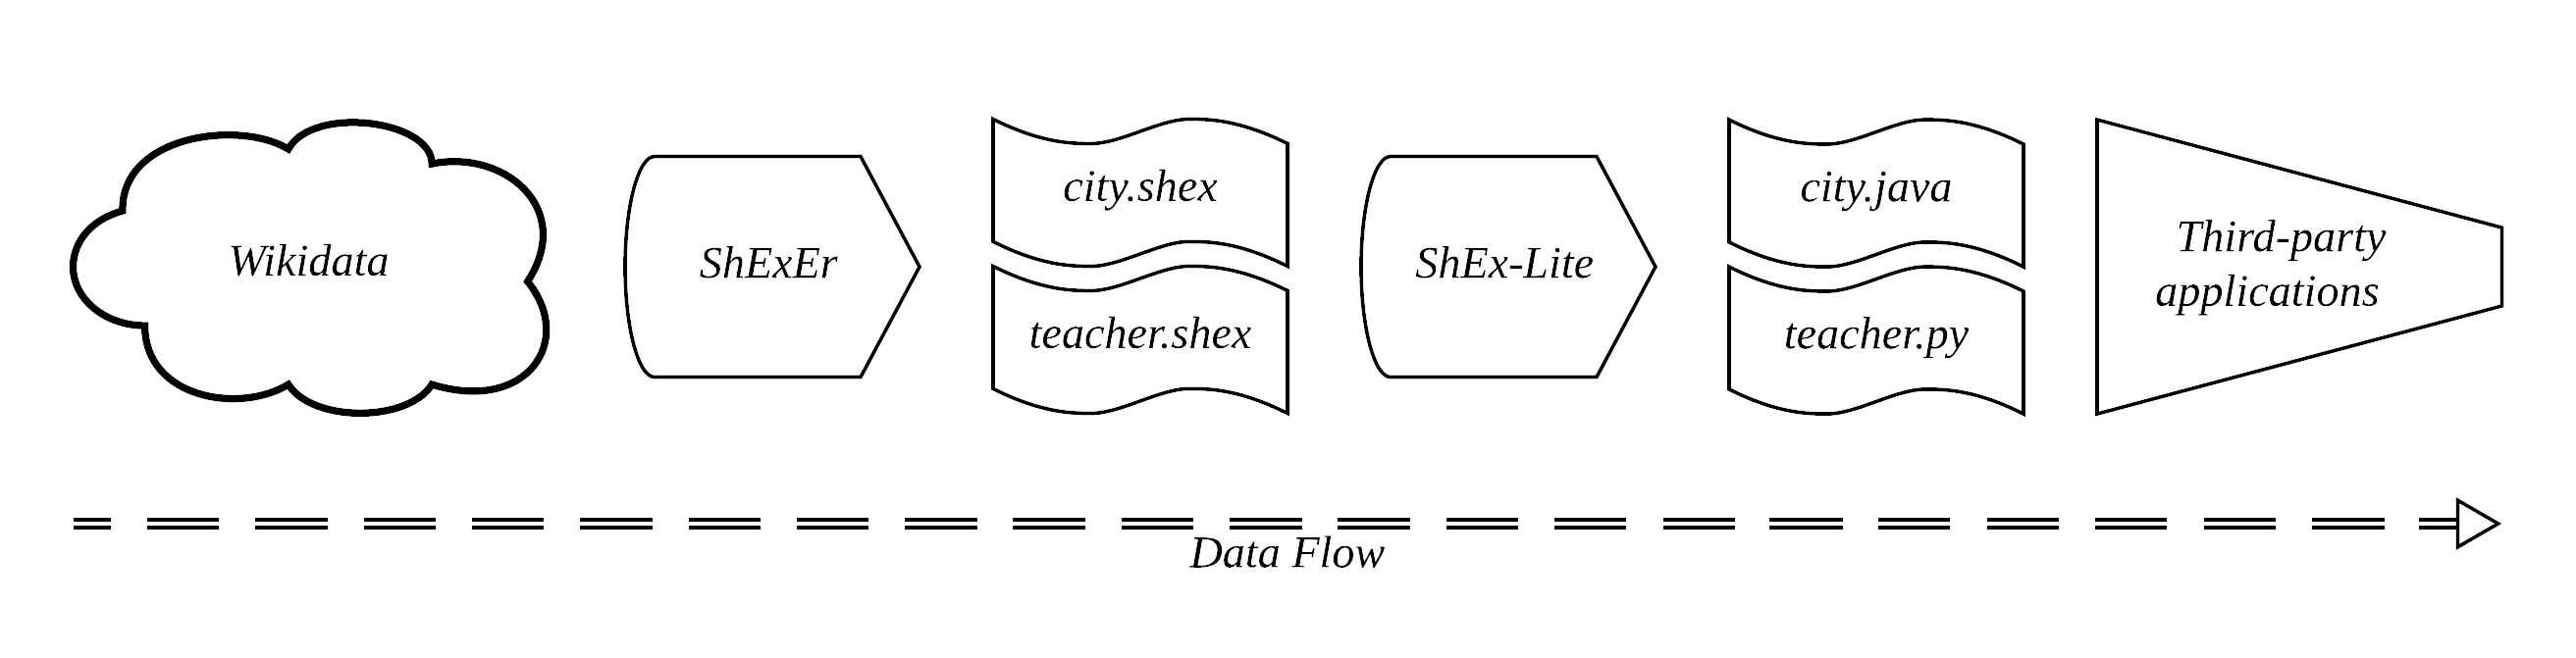
\includegraphics[width=\textwidth]{images/shex-lite-shexer-integration.png}
    \centering
    \caption[ShEx-Lite integration with Shexer]{ShEx-Lite integration with Shexer for automatically generating
    java domain object models for the Wikidata schema less existing data. This shoes the schema less data from
    wikidata from which shape expressions are inferred by shexer and later transformed to java plain objects by
    means of ShEx-Lite so third party applications can implement the domain model.}
	\label{fig:shex-lite-shexer-integration}
\end{figure}